 \documentclass[presentation]{beamer}
\usetheme{CGA}
\input{package-list-beamer}


\title[Thesis defence presentation]{Characterising antibody immunity and ageing in a short-lived teleost}
\author[William John Bradshaw]{William John Bradshaw}
\date{6th June 2019}

\def\arraystretch{1.2}
\newlength{\slideheight}
\setlength{\slideheight}{0.8\textheight}

\begin{document}

\begin{frame}
\titlepage
\end{frame}

\section{Introduction}

\subsection{B-cell immunosenescence}

\begin{frame}
\begin{figure}
\includegraphics[height=1.1\slideheight]{figs/pdf/adaptive-immunity-bcells}
\end{figure}
\end{frame}

\begin{frame}
\frametitle{Ageing has major effects on B-cell immunity}\pause
\begin{columns}
\column{0.7\textwidth}
\begin{wideitemize}{0.5}
\item Reduced na\"ive B-cell output
\item Fewer unique antibody sequences
\item Decreased responsiveness to vaccination
\item Impaired antibody quality
\item \dots
\end{wideitemize}
\end{columns}
\end{frame}

\begin{frame}
\frametitle{There's a lot we don't know about B-cell immune ageing}
\begin{columns}
\column{0.75\textwidth}\pause
\begin{wideitemize}{1}
\item Very little known outside humans and mice\pause
\item Almost all data comes from peripheral blood\pause
\item No spatial resolution (different organs)
\end{wideitemize}
\end{columns}
\end{frame}

\blackslide

\subsection{The turquoise killifish as an immunosenescence model}

\begin{frame}
\frametitle{The turquoise killifish as a model for antibody ageing}
\begin{figure}
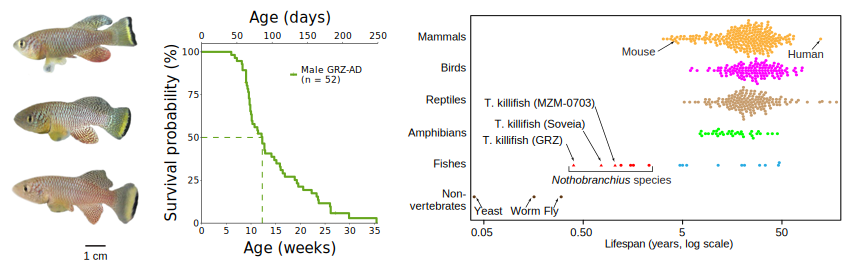
\includegraphics[width=0.9\textwidth]{figs/pdf/intro-turquoise-killifish}
\end{figure}
\end{frame}

\begin{frame}
\frametitle{How does \only<1>{B-cell immunity}\only<2->{the \textbf{antibody heavy-chain repertoire}} change with age in killifish?}
\begin{figure}
\includegraphics<2>[height=\slideheight]{figs/pdf/antibody-structure}
\includegraphics<3>[width=\textwidth]{figs/pdf/aims-1}
\includegraphics<4>[width=\textwidth]{figs/pdf/aims-2}
\includegraphics<5>[width=\textwidth]{figs/pdf/aims}
\end{figure}
\end{frame}

\begin{frame}
\frametitle{Sample design -- killifish ageing study}
\begin{figure}
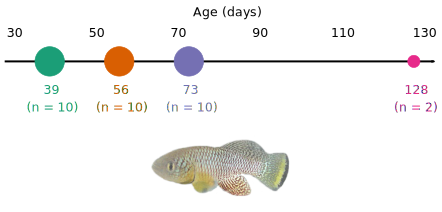
\includegraphics[width=\textwidth]{figs/pdf/design-ageing}
\end{figure}
\end{frame}

\blackslide

\begin{frame}
\frametitle{Clonal antibody diversity}
\begin{figure}
\includegraphics<2>[width=\textwidth]{figs/pdf/clonal-expansion-1}
\includegraphics<3>[width=\textwidth]{figs/pdf/clonal-expansion-2}
\includegraphics<4>[height=\slideheight]{figs/pdf/clonal-diversity-groups}
\end{figure}
\end{frame}

\section{Results}

\subsection{Killifish repertoire ageing}

\begin{frame}
\frametitle{Clonal alpha diversity in the killifish antibody repertoire \only<2->{declines with age \only<5->{at high diversity orders}}}
\begin{figure}
\includegraphics<2>[height=\slideheight]{figs/pdf/ageing-clone-diversity-alpha}
\includegraphics<3>[height=\slideheight]{figs/pdf/ageing-clone-diversity-alpha-arrow}
\includegraphics<4>[height=\slideheight]{figs/pdf/ageing-clone-diversity-alpha-arrow-lines}
\includegraphics<5>[width=0.9\textwidth]{figs/pdf/ageing-clone-diversity-solo-fit-gamma}
\end{figure}
\end{frame} % TODO: Add text for Hill numbers, reminder that 0 -> 1 = less -> more downweighting
% TODO: Add arrow showing direction of diversity change with age
% TODO: Emphasise speed of diversity loss
% TODO: Restore colour legend

\blackslide

\begin{frame}
\frametitle{\textbf{VJ} alpha diversity in the killifish antibody repertoire}
\begin{figure}
\includegraphics<1>[height=0.95\slideheight]{figs/pdf/vj-diversity-cell0}
\includegraphics<2>[height=0.95\slideheight]{figs/pdf/vj-diversity-cell1}
\includegraphics<3>[height=0.95\slideheight]{figs/pdf/vj-diversity-cell2}
\includegraphics<4>[height=0.95\slideheight]{figs/pdf/vj-diversity-cell3}
\includegraphics<5>[height=0.95\slideheight]{figs/pdf/vj-diversity-cell4}
\includegraphics<6>[height=0.95\slideheight]{figs/pdf/vj-diversity-cell5}
\includegraphics<7>[height=0.95\slideheight]{figs/pdf/vj-diversity-clones}
\includegraphics<8>[height=0.95\slideheight]{figs/pdf/vj-diversity-groups}
\end{figure}\only<9>{ }
\end{frame}

\begin{frame}
\frametitle{\textbf{VJ} alpha diversity in the killifish antibody repertoire \textbf{does not decline} with age}
\begin{figure}
\includegraphics<1>[height=0.95\slideheight]{figs/pdf/ageing-vj-diversity-alpha}
\includegraphics<2>[height=0.95\slideheight]{figs/pdf/ageing-vj-diversity-alpha-sig}
\end{figure}
\end{frame}

\begin{frame}
\frametitle{Most sequences in killifish repertoires are from small clones}
\begin{figure}
\centering

\includegraphics[height=\slideheight]{figs/pdf/ageing-pc-seq-in-small-clones}
\end{figure}
\end{frame}

\begin{frame}
\frametitle{\textbf{VJ} alpha diversity of \textbf{large clones} \only<2->{\textbf{does decline} with age}}
\begin{figure}
\includegraphics<2>[height=0.95\slideheight]{figs/pdf/ageing-vj-diversity-vlarge-alpha}
\includegraphics<3>[height=0.95\slideheight]{figs/pdf/ageing-vj-diversity-vlarge-alpha-sig}
\end{figure}
\end{frame}

\blackslide

\begin{frame}
\frametitle{Killifish VJ repertoires become \textbf{more dissimilar} with age}
\begin{figure}
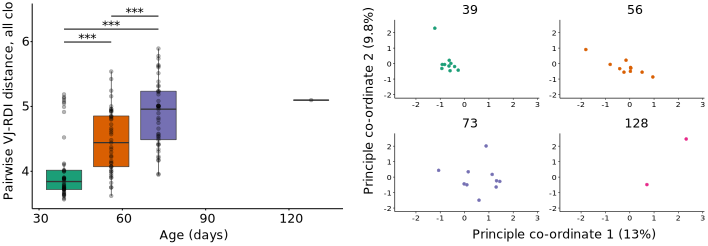
\includegraphics[height=\slideheight]{figs/pdf/ageing-rdi}
\end{figure}
\end{frame}

\begin{frame}
\frametitle{Summary I}
\begin{figure}
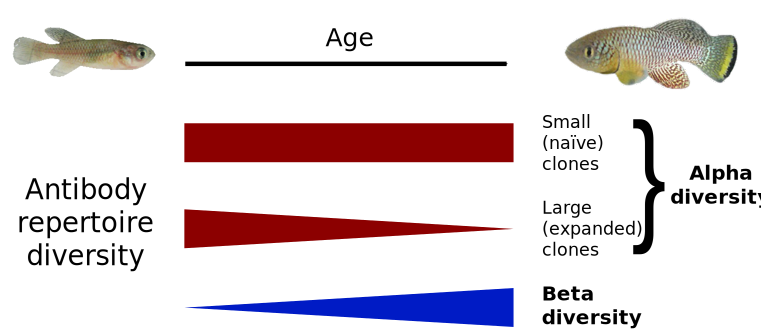
\includegraphics[width=\textwidth]{figs/pdf/graphical-summary-1}
\end{figure}
\end{frame}


\blackslide

\subsection{Intestinal repertoire ageing in the turquoise killifish}

\begin{frame}
\frametitle{Sample design -- gut repertoire study}
\begin{figure}
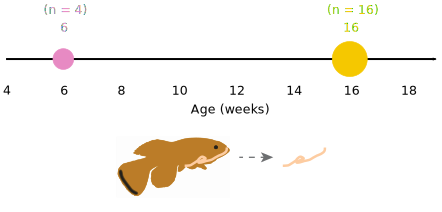
\includegraphics[width=\textwidth]{figs/pdf/design-gut}
\end{figure}
\attrib{Samples collected for Smith et al., eLife 2017}
\end{frame}

\begin{frame}
\frametitle{Killifish gut repertoires become much more dissimilar with age}
\begin{figure}
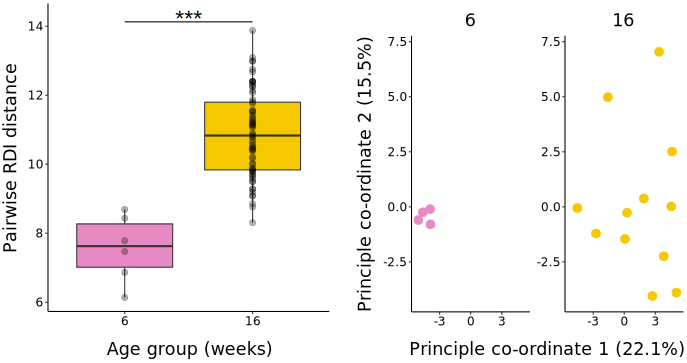
\includegraphics[height=\slideheight]{figs/pdf/igseq-gut-rdi}
\end{figure} 
\end{frame}

\begin{frame}
\frametitle{Gut repertoire alpha diversity declines dramatically with age in turquoise killifish}
\begin{figure}
\includegraphics<1,3>[width=\textwidth]{figs/pdf/igseq-gut-combined-diversity-alpha}
\includegraphics<2>[width=\textwidth]{figs/pdf/igseq-ageing-combined-diversity-alpha}
\end{figure}
\end{frame}

\begin{frame}
\frametitle{Why the difference?}
\Large
\begin{wideenum}{1}\pause
\item Difference in \textbf{environment}?\vspace{0.5em}
\begin{wideitemize}{0.5}\pause
\item Intense antigen exposure from gut microbiota
\item Greater antigen exposure $\to$ more clonal expansion, less diversity\pause
\end{wideitemize}
\item Difference in \textbf{clonal composition}?\vspace{0.5em}
\begin{wideitemize}{0.5}\pause
\item Whole body includes primary lymphoid organs, intestine does not
\item $\to$ More small na\"ive clones in whole-body samples than gut samples
\item Larger clones more age-sensitive $\to$ stronger age effect in gut samples
\end{wideitemize}
\end{wideenum}
\end{frame}

\begin{frame}
\frametitle{Killifish gut repertoires contain fewer \textbf{small} clones than whole-body repertoires}
\begin{figure}
\includegraphics[width = \textwidth]{../_Figures/png/igseq-rarefied-clone-2colour-counts-size.png}
\end{figure}
\end{frame}

\section{Summary}

\begin{frame}
% Discuss establishment of protocol etc - emphasise holistic nature of project
\frametitle{Summary II}
\begin{figure}
\includegraphics<2>[height=1.1\slideheight]{figs/pdf/graphical-summary-2a}
\includegraphics<3>[height=1.1\slideheight]{figs/pdf/graphical-summary-2b}
\includegraphics<4>[height=1.1\slideheight]{figs/pdf/graphical-summary-2c}
\end{figure}
\end{frame}

% TODO: Future directions?

\section{Acknowledgements}

\begin{frame}
\frametitle{Acknowledgements}
\small
\begin{columns}
\column{0.25\textwidth}
Dario Valenzano\\
\alert{Aleksandra Placzek}\\
\alert{Davina Patel}\\
\alert{Michael Poeschla}\\
Ray Cui\\
Joanna Dodzian\\
\alert{Pascha Hokama}\\
\alert{Lena Schlautmann}\\
\alert{Linda Zirden}\\\vspace{1.7ex}
The DV lab\\\vspace{1.7ex}
Daniela Morick\\
Doris Birker\\
Jenny Ostermann\\\vspace{1.7ex}
Aleksandra Walczak\\
B\'{e}r\'{e}nice Benayoun\\
John Beausang
\column{0.75\textwidth}
\includegraphics[width=\textwidth]{figs/jpg/group-2016}\vspace{1em}\\
\begin{columns}
\column{0.37\textwidth}
Kathrin Reichwald\\
Jason Vander Heiden\\
Quentin Marcou
\column{0.38\textwidth}
Manolis Pasparakis\\
Andreas Beyer\\
Michael L\"assig\\
\end{columns}
\end{columns}
\end{frame}
% TODO: Update picture or add Michael/Ola/Davina/etc pictures
%
% % Slide 25: Thank you and questions

\section{}
\begin{frame}\begin{center}
\Huge Thank you!
\end{center}\end{frame}


% -----------------------------------------------------------------------------


\appendix
\blackslide
\section{Extra slides}

\subsection{Background information}

\begin{frame}
\frametitle{Primary and secondary antibody diversity}
\begin{figure}
\includegraphics[height=\slideheight]{figs/pdf/bcell-repertoire-primary-secondary}
\end{figure}
\end{frame}

\begin{frame}
\frametitle{B-cell development}
\begin{figure}
\includegraphics[height=0.95\slideheight]{figs/png/b-cell-development}
\attrib{Davina Patel}
\end{figure}
\end{frame}

\begin{frame}
\frametitle{BCR signalling pathway}
\begin{figure}
\includegraphics[height=\slideheight]{figs/png/bcr-signalling}
\end{figure}
\end{frame}

\begin{frame}
\frametitle{Mechanism of VDJ recombination}
\begin{figure}
\centering
\includegraphics[height=\slideheight]{figs/pdf/extra/vdj-recombination-mechanism}
\end{figure}
\end{frame}

\begin{frame}
\frametitle{Mechanisms of junctional diversity}
\begin{figure}
\centering
\includegraphics[height=\slideheight]{figs/pdf/extra/junctional-diversity-mechanism}
\end{figure}
\end{frame}

\begin{frame}
\frametitle{Other teleost loci: simple}
\begin{figure}
\centering
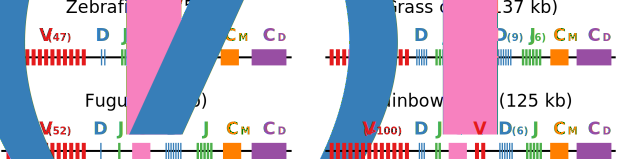
\includegraphics[width=\textwidth]{figs/pdf/extra/teleost-loci-simple}
\end{figure}
\end{frame}

\begin{frame}
\frametitle{Other teleost loci: complex}
\begin{figure}
\centering
\includegraphics[width=\textwidth]{figs/pdf/extra/teleost-loci-complex}
\end{figure}
\end{frame}


\subsection{The N. furzeri and X. maculatus IGH loci} % TODO: Add italics

\begin{frame}
\includegraphics[width=\textwidth]{figs/pdf/extra/locus-map-nfu}
\end{frame}

\begin{frame}
\includegraphics[width=\textwidth]{figs/pdf/extra/locus-map-xma}
\end{frame}

\begin{frame}
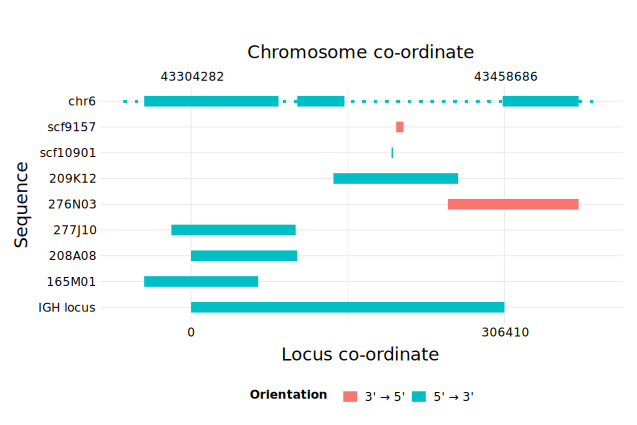
\includegraphics[width=\textwidth]{figs/pdf/extra/nfu-locus-aln}
\end{frame}

\begin{frame}
\centering
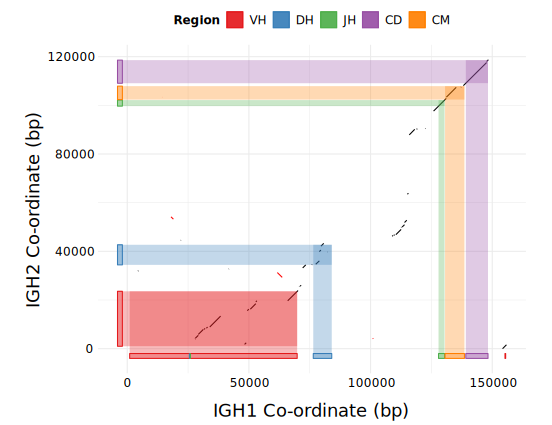
\includegraphics[width=\textheight]{figs/pdf/extra/nfu-locus-dots}
\end{frame}

\begin{frame}
\centering
\includegraphics[width=\textheight]{figs/pdf/extra/teleost-igm-exons}
\end{frame}

\begin{frame}
\centering
\includegraphics[height=\textheight]{figs/pdf/extra/ighm-sashimi-nolab}
\end{frame}

\begin{frame}
\centering
\includegraphics[height=\textheight]{figs/pdf/extra/ighd-sashimi-nolab}
\end{frame}

\begin{frame}
\centering
\includegraphics[height=\textheight]{figs/pdf/extra/ighz-sashimi-nolab}
\end{frame}

\begin{frame}
\frametitle{\textit{N. furzeri} RSS composition}
\centering
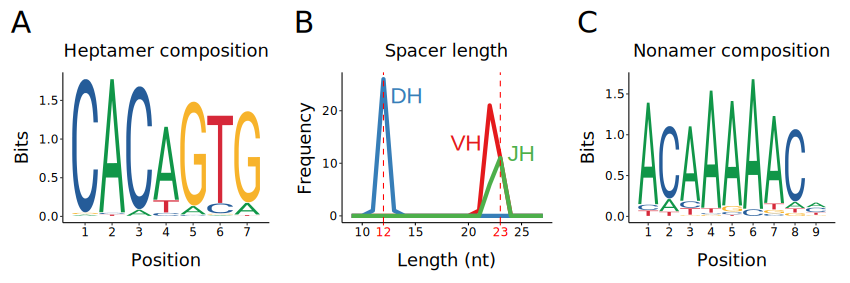
\includegraphics[width=\textwidth]{figs/pdf/extra/nfu-rss-seqlogo-all}
\end{frame}

\begin{frame}
\frametitle{\textit{X. maculatus} RSS composition}
\centering
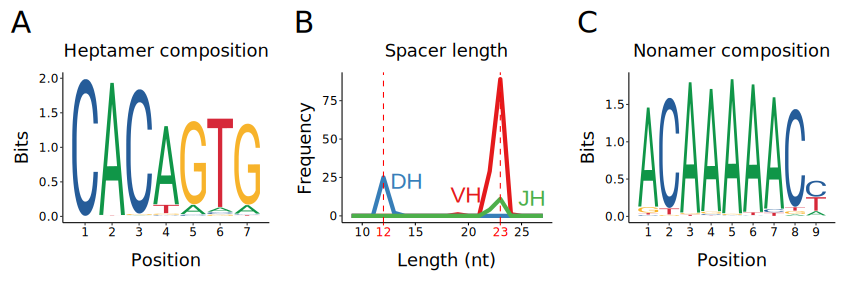
\includegraphics[width=\textwidth]{figs/pdf/extra/xma-new-rss-seqlogo-all}
\end{frame}

\subsection*{Comparative evolution of IGH loci}

\begin{frame}
\centering
\includegraphics[height=\textheight]{figs/pdf/extra/multispecies-ch-regions}
\end{frame}

\begin{frame}
\centering
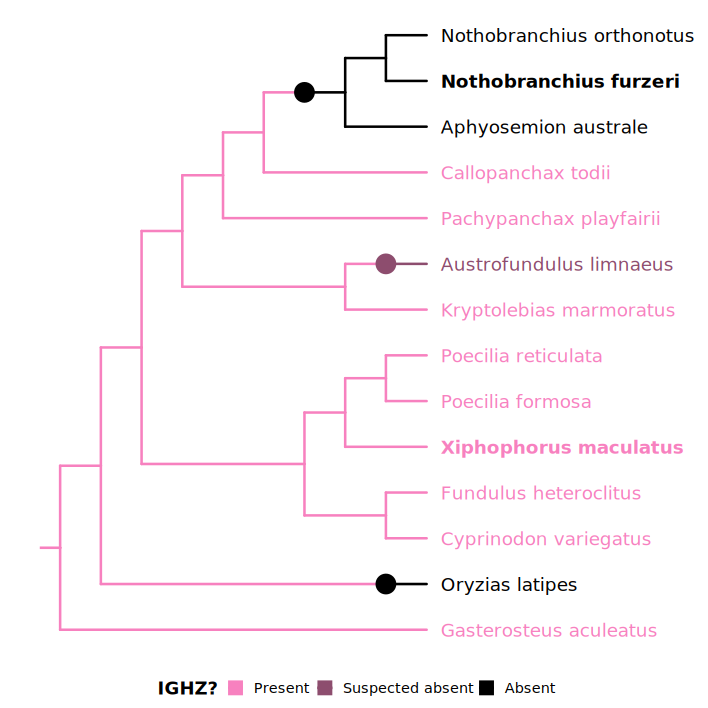
\includegraphics[height=\textheight]{figs/pdf/extra/species-tree-large-ighz}
\end{frame}

\begin{frame}
\centering
\includegraphics[height=0.9\textheight]{figs/pdf/extra/cz-trees-subclasses}
\end{frame}

\begin{frame}
\centering
\includegraphics[height=0.9\textheight]{figs/pdf/extra/cz-trees-lintree}
\end{frame}

\begin{frame}
\begin{figure}
\centering
\includegraphics[height=0.6\textheight]{figs/pdf/extra/cz-trees-ppl}
\end{figure}
\end{frame}

\begin{frame}
\begin{figure}
\centering
\includegraphics[height=0.6\textheight]{figs/pdf/extra/cz-trees-ratios}
\end{figure}
\end{frame}

\subsection{IgSeq pipelines and protocols}

\begin{frame}
\frametitle{Error correction with UMIs}
\begin{figure}
\includegraphics[height=0.9\slideheight]{figs/pdf/extra/umi-consensus}
\end{figure}
\end{frame}

\begin{frame}
\frametitle{Template switching}
\begin{figure}
\includegraphics[height=0.9\slideheight]{figs/pdf/extra/template-switch}
\end{figure}
\end{frame}

\begin{frame}
\frametitle{Bioinformatics pipeline}
\begin{figure}
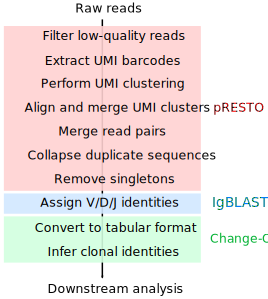
\includegraphics[height=\slideheight]{figs/pdf/immcantation-pipeline}
\end{figure}
\end{frame}

\subsection{IgSeq results}

\begin{frame}
\frametitle{Best-fit zipf distributions of pilot clonal repertoires}
\begin{figure}
\includegraphics[height=\slideheight]{figs/pdf/extra/pilot-clones-zipf-fit}
\end{figure}
\end{frame}

\begin{frame}
\frametitle{Correlation between Hill $\alpha$-spectra and other diversity metrics}
\begin{figure}
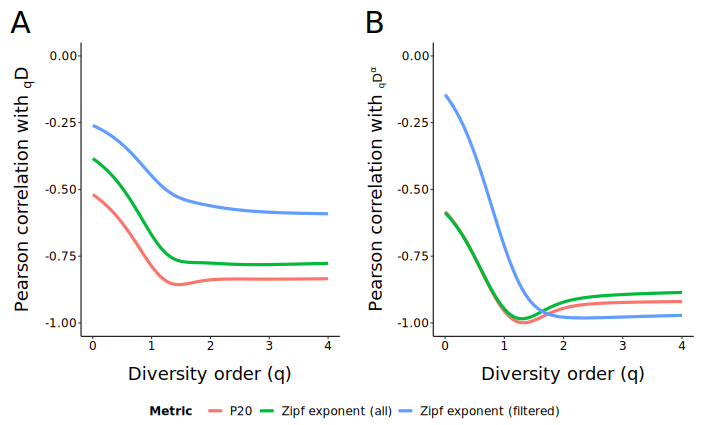
\includegraphics[height=0.95\slideheight]{figs/pdf/extra/pilot-clone-diversity-metrics-cor}
\end{figure}
\end{frame}

\begin{frame}
\frametitle{V/D/J usage probabilities in the killifish generative repertoire}
\begin{figure}
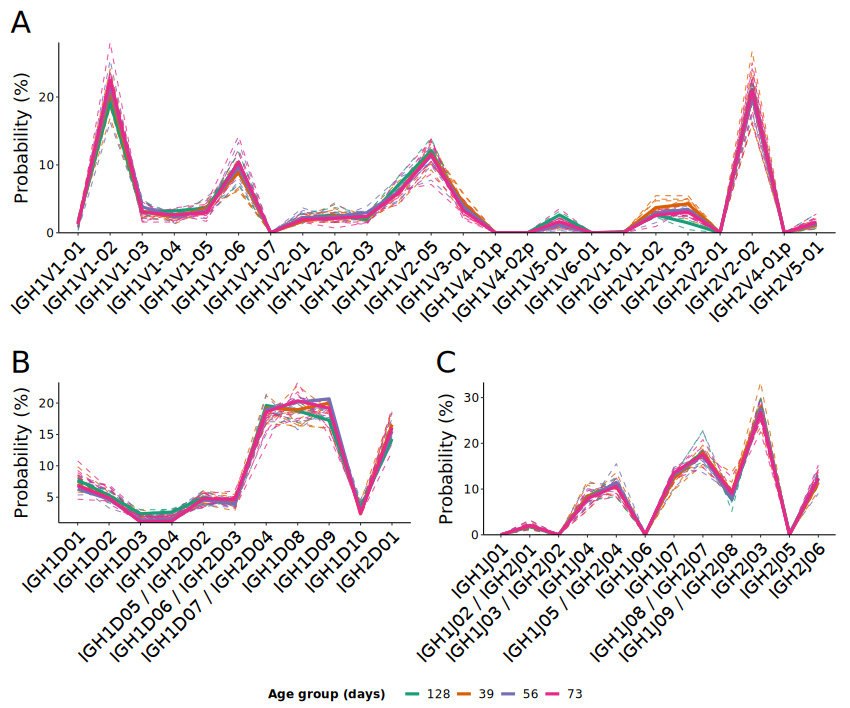
\includegraphics[height=0.95\slideheight]{figs/pdf/extra/ageing-igor-segments}
\end{figure}
\end{frame}

\begin{frame}
\frametitle{Insertion/deletion in the killifish generative repertoire}
\begin{figure}
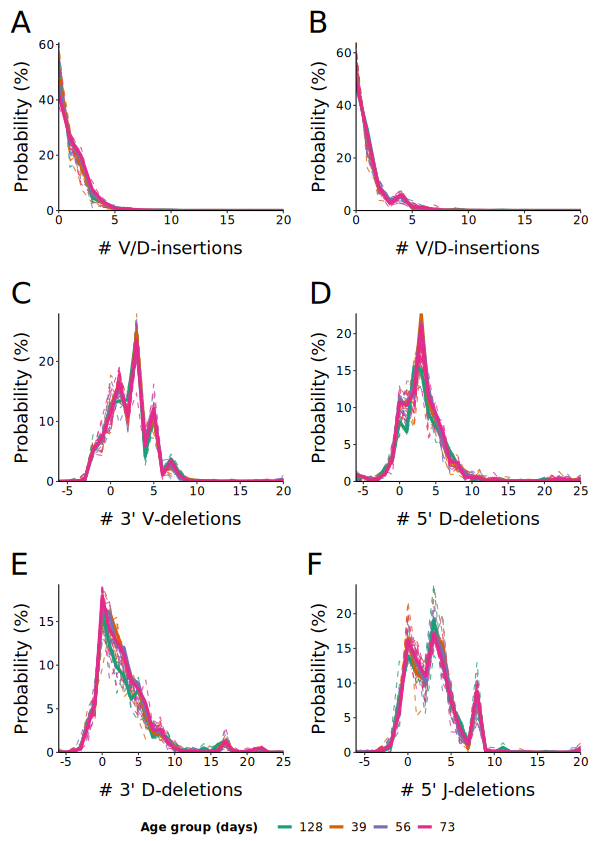
\includegraphics[height=0.95\slideheight]{figs/pdf/extra/ageing-igor-indels}
\end{figure}
\end{frame}

\begin{frame}
\frametitle{Entropy composition of the killifish generative repertoire}
\begin{figure}
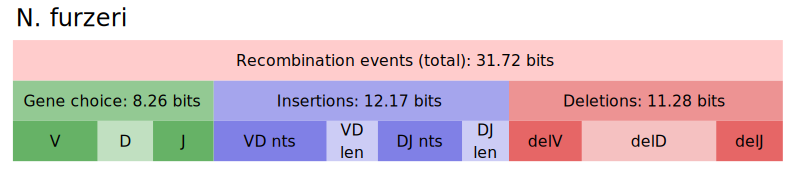
\includegraphics[width=0.9\textwidth]{figs/pdf/extra/pilot-igor-entropies}\\
\includegraphics[width=0.9\textwidth]{figs/pdf/extra/human-repertoire-entropy}
\end{figure}
\end{frame}

\begin{frame}
\frametitle{The generative entropy of the na\"ive antibody repertoire does not change with age}
\begin{figure}
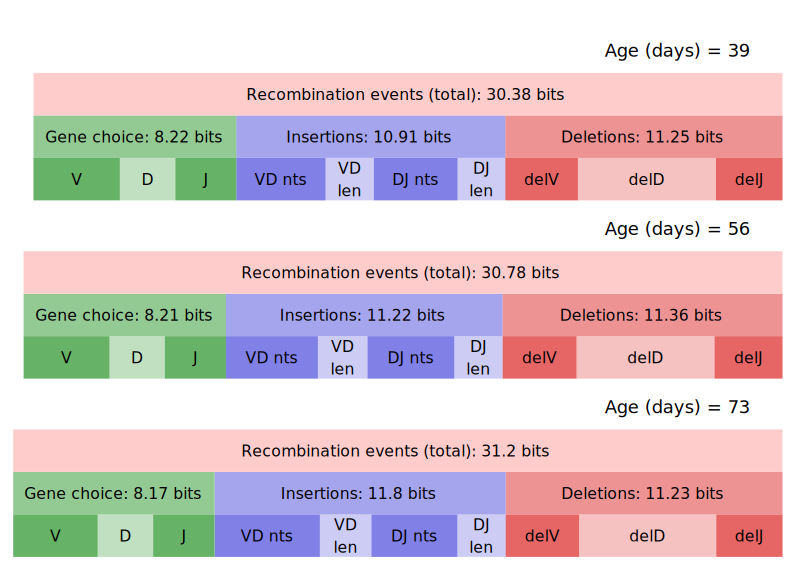
\includegraphics[height=0.95\slideheight]{figs/pdf/extra/ageing-igor-entropies}
\end{figure}
\end{frame}

\begin{frame}
\frametitle{RDI measures can reliably distinguish between individual repertoires}
\begin{figure}
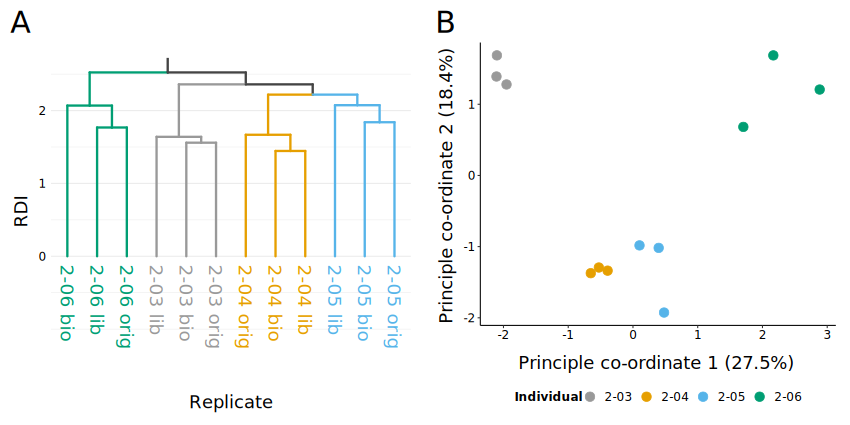
\includegraphics[width=\textwidth]{figs/pdf/extra/pilot-rdi-vj-replicate}
\end{figure}
\end{frame}

\begin{frame}
\frametitle{Most VJ combinations are dominated by small clones}
\begin{figure}
\includegraphics[height=\slideheight]{figs/pdf/vj-clonesizes}
\end{figure}
\end{frame}

\begin{frame}
\frametitle{Beta-diversity spectra: ageing cohort}
\begin{figure}
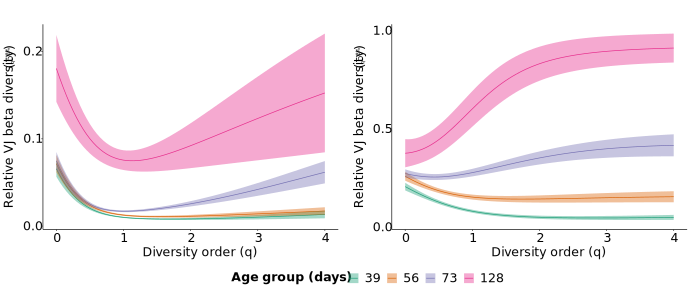
\includegraphics[width=\textwidth]{figs/pdf/ageing-vj-diversity-beta}
\end{figure}
\end{frame}

\begin{frame}
\frametitle{Gut microbiota transfer design}
\begin{figure}
\includegraphics[height=\slideheight]{figs/pdf/extra/gut-transfer-design}
\end{figure}
\end{frame}

\begin{frame}
\frametitle{Transfer-group clonal alpha diversity}
\begin{figure}
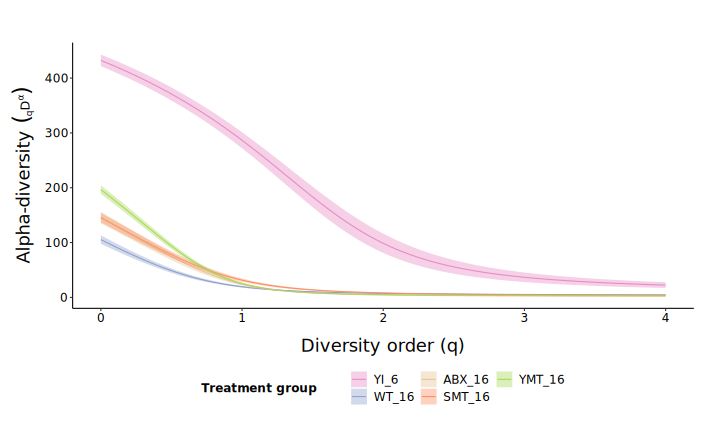
\includegraphics[height=\slideheight]{figs/pdf/extra/igseq-gut-clone-diversity-alpha-groups}
\end{figure}
\end{frame}

\begin{frame}
\frametitle{Transfer-group VJ alpha diversity}
\begin{figure}
\includegraphics[height=\slideheight]{figs/pdf/extra/igseq-gut-VJ-diversity-alpha-groups}
\end{figure}
\end{frame}

\begin{frame}
\frametitle{Transfer-group VJ beta diversity}
\begin{figure}
\includegraphics[height=\slideheight]{figs/pdf/extra/igseq-gut-VJ-diversity-beta-groups-rdi}
\end{figure}
\end{frame}

\begin{frame}
\frametitle{Beta-diversity spectra: gut samples}
\begin{figure}
\includegraphics[width=\textwidth]{figs/pdf/extra/igseq-gut-VJ-diversity-beta-spectra}
\end{figure}
\end{frame}

\begin{frame}
\frametitle{Relative rate of repertoire diversity loss}
\begin{figure}
\includegraphics[height=\slideheight]{figs/pdf/extra/comparative-diversity}
\end{figure}
\end{frame}



% TODO: Include missing IgSeq results:
% - Zipf fitting
% - Read survival
% - Correlation between measures
% - IGoR models
% - Pilot validation (inter-replicate correlation etc)
% - Effect of uBiota transfer on diversity
 
% TODO: Include Hill diversity equations and explanation

\subsection{Hill diversity}

\begin{frame}
\frametitle{Hill diversity for a unitary population $X$}
\begin{equation*}
^qD(X) = \begin{cases} \left(\displaystyle\sum_{s \in S} p_s^q \right)^{\frac{1}{1-q}} & q \neq 1\\
\exp\left(-\displaystyle\sum_{s \in S}p_s \cdot \ln p_s\right) & q = 1 \end{cases}
\end{equation*}
\end{frame}

\begin{frame}
\frametitle{Hill diversity for a structured population $C$}

\begin{equation*}
^qD_\gamma(C) = {}^qD(C)
\end{equation*}
\vfill
\begin{equation*}
^qD_\alpha(C) = \begin{cases} \left(\displaystyle\frac{1}{M}\sum_{X \in C} \left[{}^qD(X)\right]^{1-q}\right)^{\frac{1}{1-q}} & q \neq 1\\
\exp\left(\displaystyle\frac{1}{M}\sum_{X \in C} \ln {}^1D(X)\right) & q = 1 \end{cases}
\end{equation*}
\vfill
\begin{equation*}
^qD_\beta(C) = \frac{^qD_\gamma(C)}{^qD_\alpha(C)}
\end{equation*}
\end{frame}

\subsection{Burrows-Wheeler Transform}

\begin{frame}
\frametitle{Burrows-Wheeler Transform (BWT)}
\begin{figure}
\includegraphics[width=\textwidth]{figs/png/bwt}
\end{figure}
\end{frame}

\subsection{Dynamic programming alignment}

\begin{frame}
\frametitle{Needleman-Wunsch Algorithm}
\begin{figure}
\includegraphics[height=\slideheight]{figs/png/needleman-wunsch}
\end{figure}
\end{frame}

\begin{frame}
\frametitle{Smith-Waterman Algorithm}
\begin{figure}
\includegraphics[height=\slideheight]{figs/png/smith-waterman}
\end{figure}
\end{frame}

\end{document}

